\documentclass[1p]{elsarticle_modified}
%\bibliographystyle{elsarticle-num}

%\usepackage[colorlinks]{hyperref}
%\usepackage{abbrmath_seonhwa} %\Abb, \Ascr, \Acal ,\Abf, \Afrak
\usepackage{amsfonts}
\usepackage{amssymb}
\usepackage{amsmath}
\usepackage{amsthm}
\usepackage{scalefnt}
\usepackage{amsbsy}
\usepackage{kotex}
\usepackage{caption}
\usepackage{subfig}
\usepackage{color}
\usepackage{graphicx}
\usepackage{xcolor} %% white, black, red, green, blue, cyan, magenta, yellow
\usepackage{float}
\usepackage{setspace}
\usepackage{hyperref}

\usepackage{tikz}
\usetikzlibrary{arrows}

\usepackage{multirow}
\usepackage{array} % fixed length table
\usepackage{hhline}

%%%%%%%%%%%%%%%%%%%%%
\makeatletter
\renewcommand*\env@matrix[1][\arraystretch]{%
	\edef\arraystretch{#1}%
	\hskip -\arraycolsep
	\let\@ifnextchar\new@ifnextchar
	\array{*\c@MaxMatrixCols c}}
\makeatother %https://tex.stackexchange.com/questions/14071/how-can-i-increase-the-line-spacing-in-a-matrix
%%%%%%%%%%%%%%%

\usepackage[normalem]{ulem}

\newcommand{\msout}[1]{\ifmmode\text{\sout{\ensuremath{#1}}}\else\sout{#1}\fi}
%SOURCE: \msout is \stkout macro in https://tex.stackexchange.com/questions/20609/strikeout-in-math-mode

\newcommand{\cancel}[1]{
	\ifmmode
	{\color{red}\msout{#1}}
	\else
	{\color{red}\sout{#1}}
	\fi
}

\newcommand{\add}[1]{
	{\color{blue}\uwave{#1}}
}

\newcommand{\replace}[2]{
	\ifmmode
	{\color{red}\msout{#1}}{\color{blue}\uwave{#2}}
	\else
	{\color{red}\sout{#1}}{\color{blue}\uwave{#2}}
	\fi
}

\newcommand{\Sol}{\mathcal{S}} %segment
\newcommand{\D}{D} %diagram
\newcommand{\A}{\mathcal{A}} %arc


%%%%%%%%%%%%%%%%%%%%%%%%%%%%%5 test

\def\sl{\operatorname{\textup{SL}}(2,\Cbb)}
\def\psl{\operatorname{\textup{PSL}}(2,\Cbb)}
\def\quan{\mkern 1mu \triangleright \mkern 1mu}

\theoremstyle{definition}
\newtheorem{thm}{Theorem}[section]
\newtheorem{prop}[thm]{Proposition}
\newtheorem{lem}[thm]{Lemma}
\newtheorem{ques}[thm]{Question}
\newtheorem{cor}[thm]{Corollary}
\newtheorem{defn}[thm]{Definition}
\newtheorem{exam}[thm]{Example}
\newtheorem{rmk}[thm]{Remark}
\newtheorem{alg}[thm]{Algorithm}

\newcommand{\I}{\sqrt{-1}}
\begin{document}

%\begin{frontmatter}
%
%\title{Boundary parabolic representations of knots up to 8 crossings}
%
%%% Group authors per affiliation:
%\author{Yunhi Cho} 
%\address{Department of Mathematics, University of Seoul, Seoul, Korea}
%\ead{yhcho@uos.ac.kr}
%
%
%\author{Seonhwa Kim} %\fnref{s_kim}}
%\address{Center for Geometry and Physics, Institute for Basic Science, Pohang, 37673, Korea}
%\ead{ryeona17@ibs.re.kr}
%
%\author{Hyuk Kim}
%\address{Department of Mathematical Sciences, Seoul National University, Seoul 08826, Korea}
%\ead{hyukkim@snu.ac.kr}
%
%\author{Seokbeom Yoon}
%\address{Department of Mathematical Sciences, Seoul National University, Seoul, 08826,  Korea}
%\ead{sbyoon15@snu.ac.kr}
%
%\begin{abstract}
%We find all boundary parabolic representation of knots up to 8 crossings.
%
%\end{abstract}
%\begin{keyword}
%    \MSC[2010] 57M25 
%\end{keyword}
%
%\end{frontmatter}

%\linenumbers
%\tableofcontents
%
\newcommand\colored[1]{\textcolor{white}{\rule[-0.35ex]{0.8em}{1.4ex}}\kern-0.8em\color{red} #1}%
%\newcommand\colored[1]{\textcolor{white}{ #1}\kern-2.17ex	\textcolor{white}{ #1}\kern-1.81ex	\textcolor{white}{ #1}\kern-2.15ex\color{red}#1	}

{\Large $\underline{11n_{124}~(K11n_{124})}$}

\setlength{\tabcolsep}{10pt}
\renewcommand{\arraystretch}{1.6}
\vspace{1cm}\begin{tabular}{m{100pt}>{\centering\arraybackslash}m{274pt}}
\multirow{5}{120pt}{
	\centering
	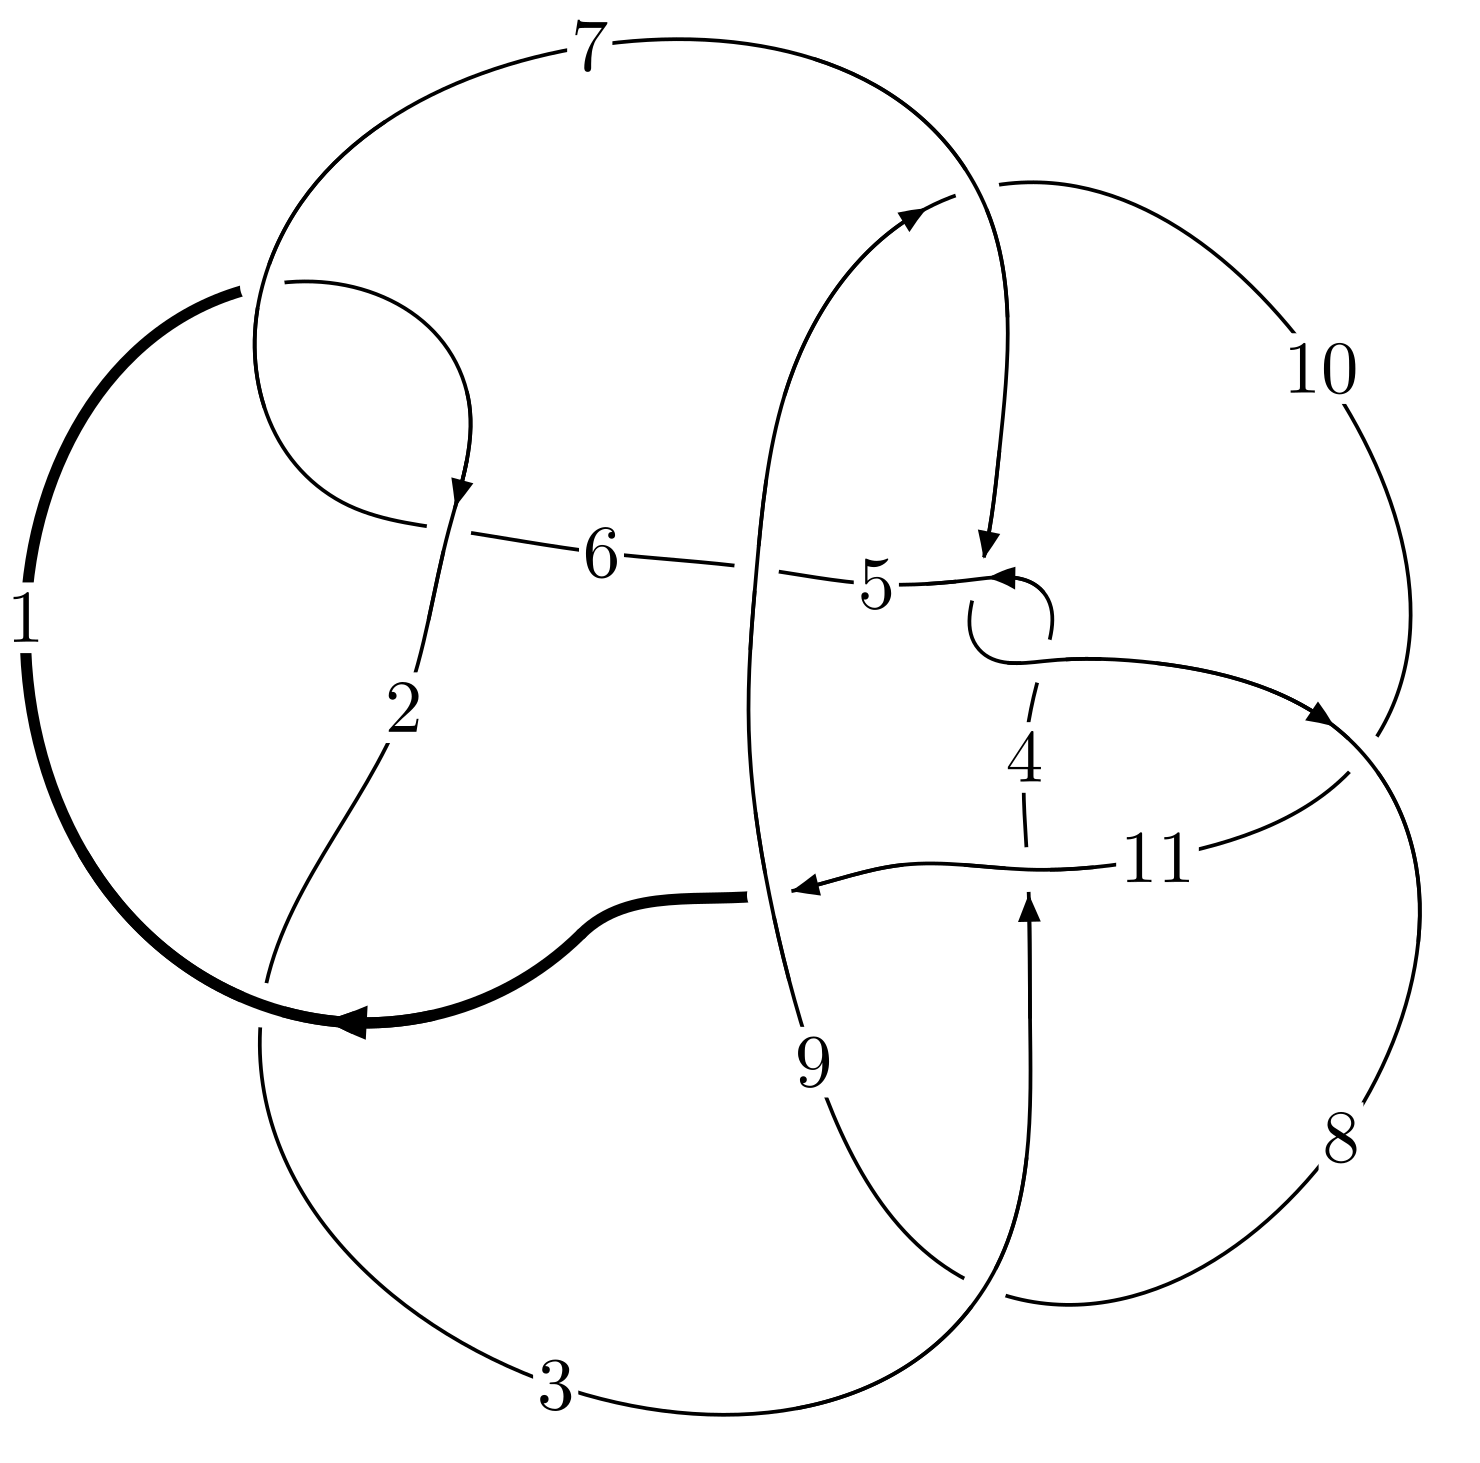
\includegraphics[width=112pt]{../../../GIT/diagram.site/Diagrams/png/740_11n_124.png}\\
\ \ \ A knot diagram\footnotemark}&
\allowdisplaybreaks
\textbf{Linearized knot diagam} \\
\cline{2-2}
 &
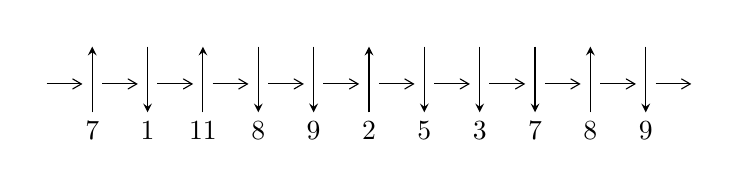
\begin{tikzpicture}[x=20pt, y=17pt]
	% nodes
	\node (C0) at (0, 0) {};
	\node (C1) at (1, 0) {};
	\node (C1U) at (1, +1) {};
	\node (C1D) at (1, -1) {7};

	\node (C2) at (2, 0) {};
	\node (C2U) at (2, +1) {};
	\node (C2D) at (2, -1) {1};

	\node (C3) at (3, 0) {};
	\node (C3U) at (3, +1) {};
	\node (C3D) at (3, -1) {11};

	\node (C4) at (4, 0) {};
	\node (C4U) at (4, +1) {};
	\node (C4D) at (4, -1) {8};

	\node (C5) at (5, 0) {};
	\node (C5U) at (5, +1) {};
	\node (C5D) at (5, -1) {9};

	\node (C6) at (6, 0) {};
	\node (C6U) at (6, +1) {};
	\node (C6D) at (6, -1) {2};

	\node (C7) at (7, 0) {};
	\node (C7U) at (7, +1) {};
	\node (C7D) at (7, -1) {5};

	\node (C8) at (8, 0) {};
	\node (C8U) at (8, +1) {};
	\node (C8D) at (8, -1) {3};

	\node (C9) at (9, 0) {};
	\node (C9U) at (9, +1) {};
	\node (C9D) at (9, -1) {7};

	\node (C10) at (10, 0) {};
	\node (C10U) at (10, +1) {};
	\node (C10D) at (10, -1) {8};

	\node (C11) at (11, 0) {};
	\node (C11U) at (11, +1) {};
	\node (C11D) at (11, -1) {9};
	\node (C12) at (12, 0) {};

	% arrows
	\draw[->,>={angle 60}]
	(C0) edge (C1) (C1) edge (C2) (C2) edge (C3) (C3) edge (C4) (C4) edge (C5) (C5) edge (C6) (C6) edge (C7) (C7) edge (C8) (C8) edge (C9) (C9) edge (C10) (C10) edge (C11) (C11) edge (C12) ;	\draw[->,>=stealth]
	(C1D) edge (C1U) (C2U) edge (C2D) (C3D) edge (C3U) (C4U) edge (C4D) (C5U) edge (C5D) (C6D) edge (C6U) (C7U) edge (C7D) (C8U) edge (C8D) (C9U) edge (C9D) (C10D) edge (C10U) (C11U) edge (C11D) ;
	\end{tikzpicture} \\
\hhline{~~} \\& 
\textbf{Solving Sequence} \\ \cline{2-2} 
 &
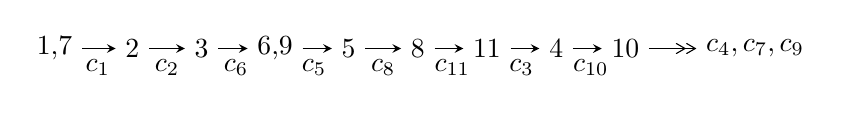
\begin{tikzpicture}[x=25pt, y=7pt]
	% node
	\node (A0) at (-1/8, 0) {1,7};
	\node (A1) at (1, 0) {2};
	\node (A2) at (2, 0) {3};
	\node (A3) at (49/16, 0) {6,9};
	\node (A4) at (33/8, 0) {5};
	\node (A5) at (41/8, 0) {8};
	\node (A6) at (49/8, 0) {11};
	\node (A7) at (57/8, 0) {4};
	\node (A8) at (65/8, 0) {10};
	\node (C1) at (1/2, -1) {$c_{1}$};
	\node (C2) at (3/2, -1) {$c_{2}$};
	\node (C3) at (5/2, -1) {$c_{6}$};
	\node (C4) at (29/8, -1) {$c_{5}$};
	\node (C5) at (37/8, -1) {$c_{8}$};
	\node (C6) at (45/8, -1) {$c_{11}$};
	\node (C7) at (53/8, -1) {$c_{3}$};
	\node (C8) at (61/8, -1) {$c_{10}$};
	\node (A9) at (10, 0) {$c_{4},c_{7},c_{9}$};

	% edge
	\draw[->,>=stealth]	
	(A0) edge (A1) (A1) edge (A2) (A2) edge (A3) (A3) edge (A4) (A4) edge (A5) (A5) edge (A6) (A6) edge (A7) (A7) edge (A8) ;
	\draw[->>,>={angle 60}]	
	(A8) edge (A9);
\end{tikzpicture} \\ 

\end{tabular} \\

\footnotetext{
The image of knot diagram is generated by the software ``\textbf{Draw programme}" developed by Andrew Bartholomew(\url{http://www.layer8.co.uk/maths/draw/index.htm\#Running-draw}), where we modified some parts for our purpose(\url{https://github.com/CATsTAILs/LinksPainter}).
}\phantom \\ \newline 
\centering \textbf{Ideals for irreducible components\footnotemark of $X_{\text{par}}$} 
 
\begin{align*}
I^u_{1}&=\langle 
1.78739\times10^{29} u^{38}-5.50902\times10^{28} u^{37}+\cdots+1.67323\times10^{29} b+1.20675\times10^{29},\\
\phantom{I^u_{1}}&\phantom{= \langle  }-1.82393\times10^{30} u^{38}+7.78408\times10^{29} u^{37}+\cdots+1.17126\times10^{30} a+1.39048\times10^{30},\\
\phantom{I^u_{1}}&\phantom{= \langle  }u^{39}+12 u^{37}+\cdots+14 u+7\rangle \\
I^u_{2}&=\langle 
- u^9-2 u^7-4 u^5-4 u^3+u^2+b-3 u+1,\;- u^9- u^8-2 u^7- u^6-3 u^5-2 u^4-3 u^3+a- u-1,\\
\phantom{I^u_{2}}&\phantom{= \langle  }u^{10}+u^9+3 u^8+2 u^7+5 u^6+3 u^5+6 u^4+2 u^3+4 u^2+u+1\rangle \\
\\
\end{align*}
\raggedright * 2 irreducible components of $\dim_{\mathbb{C}}=0$, with total 49 representations.\\
\footnotetext{All coefficients of polynomials are rational numbers. But the coefficients are sometimes approximated in decimal forms when there is not enough margin.}
\newpage
\renewcommand{\arraystretch}{1}
\centering \section*{I. $I^u_{1}= \langle 1.79\times10^{29} u^{38}-5.51\times10^{28} u^{37}+\cdots+1.67\times10^{29} b+1.21\times10^{29},\;-1.82\times10^{30} u^{38}+7.78\times10^{29} u^{37}+\cdots+1.17\times10^{30} a+1.39\times10^{30},\;u^{39}+12 u^{37}+\cdots+14 u+7 \rangle$}
\flushleft \textbf{(i) Arc colorings}\\
\begin{tabular}{m{7pt} m{180pt} m{7pt} m{180pt} }
\flushright $a_{1}=$&$\begin{pmatrix}1\\0\end{pmatrix}$ \\
\flushright $a_{7}=$&$\begin{pmatrix}0\\u\end{pmatrix}$ \\
\flushright $a_{2}=$&$\begin{pmatrix}1\\- u^2\end{pmatrix}$ \\
\flushright $a_{3}=$&$\begin{pmatrix}u^2+1\\- u^2\end{pmatrix}$ \\
\flushright $a_{6}=$&$\begin{pmatrix}- u\\u^3+u\end{pmatrix}$ \\
\flushright $a_{9}=$&$\begin{pmatrix}1.55724 u^{38}-0.664589 u^{37}+\cdots+7.55322 u-1.18716\\-1.06823 u^{38}+0.329244 u^{37}+\cdots-6.46213 u-0.721210\end{pmatrix}$ \\
\flushright $a_{5}=$&$\begin{pmatrix}0.737177 u^{38}+0.407586 u^{37}+\cdots+13.5161 u+4.88745\\-2.22063 u^{38}-0.382128 u^{37}+\cdots-28.9097 u-7.31310\end{pmatrix}$ \\
\flushright $a_{8}=$&$\begin{pmatrix}1.34253 u^{38}-0.801447 u^{37}+\cdots+4.38094 u-2.85956\\-2.08428 u^{38}+0.937331 u^{37}+\cdots-8.48023 u+2.57739\end{pmatrix}$ \\
\flushright $a_{11}=$&$\begin{pmatrix}0.596770 u^{38}-0.670897 u^{37}+\cdots-3.69102 u-2.60571\\-1.27517 u^{38}+2.12949 u^{37}+\cdots+15.8112 u+14.1929\end{pmatrix}$ \\
\flushright $a_{4}=$&$\begin{pmatrix}-0.639576 u^{38}+0.925361 u^{37}+\cdots+6.56459 u+5.74668\\2.68940 u^{38}-1.07792 u^{37}+\cdots+15.6841 u-1.72061\end{pmatrix}$ \\
\flushright $a_{10}=$&$\begin{pmatrix}1.55724 u^{38}-0.664589 u^{37}+\cdots+7.55322 u-1.18716\\-2.21877 u^{38}+1.13010 u^{37}+\cdots-8.05855 u+3.93091\end{pmatrix}$\\ \flushright $a_{10}=$&$\begin{pmatrix}1.55724 u^{38}-0.664589 u^{37}+\cdots+7.55322 u-1.18716\\-2.21877 u^{38}+1.13010 u^{37}+\cdots-8.05855 u+3.93091\end{pmatrix}$\\&\end{tabular}
\flushleft \textbf{(ii) Obstruction class $= -1$}\\~\\
\flushleft \textbf{(iii) Cusp Shapes $= 3.03813 u^{38}-1.76931 u^{37}+\cdots+10.1449 u-9.34970$}\\~\\
\newpage\renewcommand{\arraystretch}{1}
\flushleft \textbf{(iv) u-Polynomials at the component}\newline \\
\begin{tabular}{m{50pt}|m{274pt}}
Crossings & \hspace{64pt}u-Polynomials at each crossing \\
\hline $$\begin{aligned}c_{1},c_{6}\end{aligned}$$&$\begin{aligned}
&u^{39}+12 u^{37}+\cdots+14 u+7
\end{aligned}$\\
\hline $$\begin{aligned}c_{2}\end{aligned}$$&$\begin{aligned}
&u^{39}+24 u^{38}+\cdots-280 u-49
\end{aligned}$\\
\hline $$\begin{aligned}c_{3}\end{aligned}$$&$\begin{aligned}
&u^{39}+3 u^{38}+\cdots+9 u+1
\end{aligned}$\\
\hline $$\begin{aligned}c_{4},c_{7}\end{aligned}$$&$\begin{aligned}
&u^{39}-3 u^{38}+\cdots-9 u+1
\end{aligned}$\\
\hline $$\begin{aligned}c_{5}\end{aligned}$$&$\begin{aligned}
&u^{39}+u^{38}+\cdots-1365 u+253
\end{aligned}$\\
\hline $$\begin{aligned}c_{8}\end{aligned}$$&$\begin{aligned}
&u^{39}+u^{38}+\cdots-11 u+1
\end{aligned}$\\
\hline $$\begin{aligned}c_{9}\end{aligned}$$&$\begin{aligned}
&u^{39}- u^{38}+\cdots-265 u+47
\end{aligned}$\\
\hline $$\begin{aligned}c_{10}\end{aligned}$$&$\begin{aligned}
&u^{39}+3 u^{38}+\cdots-19 u+1
\end{aligned}$\\
\hline $$\begin{aligned}c_{11}\end{aligned}$$&$\begin{aligned}
&u^{39}- u^{38}+\cdots+90 u+209
\end{aligned}$\\
\hline
\end{tabular}\\~\\
\newpage\renewcommand{\arraystretch}{1}
\flushleft \textbf{(v) Riley Polynomials at the component}\newline \\
\begin{tabular}{m{50pt}|m{274pt}}
Crossings & \hspace{64pt}Riley Polynomials at each crossing \\
\hline $$\begin{aligned}c_{1},c_{6}\end{aligned}$$&$\begin{aligned}
&y^{39}+24 y^{38}+\cdots-280 y-49
\end{aligned}$\\
\hline $$\begin{aligned}c_{2}\end{aligned}$$&$\begin{aligned}
&y^{39}-12 y^{38}+\cdots-29400 y-2401
\end{aligned}$\\
\hline $$\begin{aligned}c_{3}\end{aligned}$$&$\begin{aligned}
&y^{39}+35 y^{38}+\cdots-63 y-1
\end{aligned}$\\
\hline $$\begin{aligned}c_{4},c_{7}\end{aligned}$$&$\begin{aligned}
&y^{39}+y^{38}+\cdots+37 y-1
\end{aligned}$\\
\hline $$\begin{aligned}c_{5}\end{aligned}$$&$\begin{aligned}
&y^{39}-43 y^{38}+\cdots-1224387 y-64009
\end{aligned}$\\
\hline $$\begin{aligned}c_{8}\end{aligned}$$&$\begin{aligned}
&y^{39}+9 y^{38}+\cdots+31 y-1
\end{aligned}$\\
\hline $$\begin{aligned}c_{9}\end{aligned}$$&$\begin{aligned}
&y^{39}-37 y^{38}+\cdots+14483 y-2209
\end{aligned}$\\
\hline $$\begin{aligned}c_{10}\end{aligned}$$&$\begin{aligned}
&y^{39}+39 y^{38}+\cdots-61 y-1
\end{aligned}$\\
\hline $$\begin{aligned}c_{11}\end{aligned}$$&$\begin{aligned}
&y^{39}-23 y^{38}+\cdots+796448 y-43681
\end{aligned}$\\
\hline
\end{tabular}\\~\\
\newpage\flushleft \textbf{(vi) Complex Volumes and Cusp Shapes}
$$\begin{array}{c|c|c}  
\text{Solutions to }I^u_{1}& \I (\text{vol} + \sqrt{-1}CS) & \text{Cusp shape}\\
 \hline 
\begin{aligned}
u &= \phantom{-}0.970374 + 0.165160 I \\
a &= -1.38216 + 0.38547 I \\
b &= \phantom{-}1.298900 + 0.346398 I\end{aligned}
 & -5.72155 + 0.54332 I & -4.48404 - 0.44801 I \\ \hline\begin{aligned}
u &= \phantom{-}0.970374 - 0.165160 I \\
a &= -1.38216 - 0.38547 I \\
b &= \phantom{-}1.298900 - 0.346398 I\end{aligned}
 & -5.72155 - 0.54332 I & -4.48404 + 0.44801 I \\ \hline\begin{aligned}
u &= -0.145422 + 0.960485 I \\
a &= -0.312403 + 1.125530 I \\
b &= -0.75018 - 1.96873 I\end{aligned}
 & -2.60397 - 3.58012 I & -5.99936 + 4.69227 I \\ \hline\begin{aligned}
u &= -0.145422 - 0.960485 I \\
a &= -0.312403 - 1.125530 I \\
b &= -0.75018 + 1.96873 I\end{aligned}
 & -2.60397 + 3.58012 I & -5.99936 - 4.69227 I \\ \hline\begin{aligned}
u &= \phantom{-}0.244496 + 0.924229 I \\
a &= \phantom{-}0.771798 + 0.143039 I \\
b &= \phantom{-}0.389292 - 0.068286 I\end{aligned}
 & -0.62997 + 1.59285 I & -3.23591 - 4.35949 I \\ \hline\begin{aligned}
u &= \phantom{-}0.244496 - 0.924229 I \\
a &= \phantom{-}0.771798 - 0.143039 I \\
b &= \phantom{-}0.389292 + 0.068286 I\end{aligned}
 & -0.62997 - 1.59285 I & -3.23591 + 4.35949 I \\ \hline\begin{aligned}
u &= -0.075811 + 0.941393 I \\
a &= -0.57379 - 1.58798 I \\
b &= -0.680895 + 0.570692 I\end{aligned}
 & \phantom{-}1.322390 - 0.422831 I & -4.94003 - 1.41438 I \\ \hline\begin{aligned}
u &= -0.075811 - 0.941393 I \\
a &= -0.57379 + 1.58798 I \\
b &= -0.680895 - 0.570692 I\end{aligned}
 & \phantom{-}1.322390 + 0.422831 I & -4.94003 + 1.41438 I \\ \hline\begin{aligned}
u &= -1.067820 + 0.145596 I \\
a &= -1.383670 + 0.195517 I \\
b &= \phantom{-}1.253910 - 0.603680 I\end{aligned}
 & -5.61750 + 7.80414 I & -3.64994 - 4.73695 I \\ \hline\begin{aligned}
u &= -1.067820 - 0.145596 I \\
a &= -1.383670 - 0.195517 I \\
b &= \phantom{-}1.253910 + 0.603680 I\end{aligned}
 & -5.61750 - 7.80414 I & -3.64994 + 4.73695 I\\
 \hline 
 \end{array}$$\newpage$$\begin{array}{c|c|c}  
\text{Solutions to }I^u_{1}& \I (\text{vol} + \sqrt{-1}CS) & \text{Cusp shape}\\
 \hline 
\begin{aligned}
u &= -0.661560 + 0.856108 I \\
a &= -0.105096 - 0.363168 I \\
b &= \phantom{-}1.104730 - 0.357036 I\end{aligned}
 & \phantom{-}5.00877 - 2.57683 I & \phantom{-}6.58497 + 2.64677 I \\ \hline\begin{aligned}
u &= -0.661560 - 0.856108 I \\
a &= -0.105096 + 0.363168 I \\
b &= \phantom{-}1.104730 + 0.357036 I\end{aligned}
 & \phantom{-}5.00877 + 2.57683 I & \phantom{-}6.58497 - 2.64677 I \\ \hline\begin{aligned}
u &= -0.365080 + 1.061570 I \\
a &= -1.16765 + 0.98033 I \\
b &= -0.986442 - 0.985917 I\end{aligned}
 & -2.63598 - 6.13265 I & -3.84561 + 9.40841 I \\ \hline\begin{aligned}
u &= -0.365080 - 1.061570 I \\
a &= -1.16765 - 0.98033 I \\
b &= -0.986442 + 0.985917 I\end{aligned}
 & -2.63598 + 6.13265 I & -3.84561 - 9.40841 I \\ \hline\begin{aligned}
u &= \phantom{-}0.518178 + 0.693040 I \\
a &= \phantom{-}0.925341 - 0.451847 I \\
b &= -0.197420 + 0.429722 I\end{aligned}
 & \phantom{-}0.23938 + 2.14007 I & -2.40854 - 4.03571 I \\ \hline\begin{aligned}
u &= \phantom{-}0.518178 - 0.693040 I \\
a &= \phantom{-}0.925341 + 0.451847 I \\
b &= -0.197420 - 0.429722 I\end{aligned}
 & \phantom{-}0.23938 - 2.14007 I & -2.40854 + 4.03571 I \\ \hline\begin{aligned}
u &= -0.358275 + 0.727858 I \\
a &= \phantom{-}1.31473 + 0.56113 I \\
b &= -0.235788 + 1.229960 I\end{aligned}
 & -2.12535 + 1.41634 I & -6.42200 + 1.56979 I \\ \hline\begin{aligned}
u &= -0.358275 - 0.727858 I \\
a &= \phantom{-}1.31473 - 0.56113 I \\
b &= -0.235788 - 1.229960 I\end{aligned}
 & -2.12535 - 1.41634 I & -6.42200 - 1.56979 I \\ \hline\begin{aligned}
u &= \phantom{-}0.142576 + 1.181590 I \\
a &= -0.256537 + 0.091644 I \\
b &= -1.63516 + 0.43597 I\end{aligned}
 & -4.72844 + 2.99253 I & -9.56242 - 1.88756 I \\ \hline\begin{aligned}
u &= \phantom{-}0.142576 - 1.181590 I \\
a &= -0.256537 - 0.091644 I \\
b &= -1.63516 - 0.43597 I\end{aligned}
 & -4.72844 - 2.99253 I & -9.56242 + 1.88756 I\\
 \hline 
 \end{array}$$\newpage$$\begin{array}{c|c|c}  
\text{Solutions to }I^u_{1}& \I (\text{vol} + \sqrt{-1}CS) & \text{Cusp shape}\\
 \hline 
\begin{aligned}
u &= -0.461639 + 1.163800 I \\
a &= \phantom{-}0.093896 + 1.347320 I \\
b &= -1.63447 - 0.73754 I\end{aligned}
 & -4.83553 - 4.15063 I & -11.12509 + 1.85834 I \\ \hline\begin{aligned}
u &= -0.461639 - 1.163800 I \\
a &= \phantom{-}0.093896 - 1.347320 I \\
b &= -1.63447 + 0.73754 I\end{aligned}
 & -4.83553 + 4.15063 I & -11.12509 - 1.85834 I \\ \hline\begin{aligned}
u &= \phantom{-}0.861374 + 0.909425 I \\
a &= \phantom{-}0.420286 - 0.450008 I \\
b &= -0.526827 - 0.046250 I\end{aligned}
 & \phantom{-}0.74799 + 3.17123 I & -8.85439 - 3.48619 I \\ \hline\begin{aligned}
u &= \phantom{-}0.861374 - 0.909425 I \\
a &= \phantom{-}0.420286 + 0.450008 I \\
b &= -0.526827 + 0.046250 I\end{aligned}
 & \phantom{-}0.74799 - 3.17123 I & -8.85439 + 3.48619 I \\ \hline\begin{aligned}
u &= \phantom{-}0.715910 + 0.207951 I \\
a &= \phantom{-}0.864160 - 0.809698 I \\
b &= -0.363007 + 0.664118 I\end{aligned}
 & \phantom{-}1.08867 + 1.79567 I & \phantom{-}3.61269 - 3.73862 I \\ \hline\begin{aligned}
u &= \phantom{-}0.715910 - 0.207951 I \\
a &= \phantom{-}0.864160 + 0.809698 I \\
b &= -0.363007 - 0.664118 I\end{aligned}
 & \phantom{-}1.08867 - 1.79567 I & \phantom{-}3.61269 + 3.73862 I \\ \hline\begin{aligned}
u &= -0.660029\phantom{ +0.000000I} \\
a &= \phantom{-}1.75790\phantom{ +0.000000I} \\
b &= -0.957650\phantom{ +0.000000I}\end{aligned}
 & -1.67672\phantom{ +0.000000I} & -6.74230\phantom{ +0.000000I} \\ \hline\begin{aligned}
u &= \phantom{-}0.399747 + 1.326200 I \\
a &= -0.135365 + 1.304920 I \\
b &= \phantom{-}1.029460 - 0.406010 I\end{aligned}
 & -10.43670 + 5.23929 I & -7.47031 - 3.45363 I \\ \hline\begin{aligned}
u &= \phantom{-}0.399747 - 1.326200 I \\
a &= -0.135365 - 1.304920 I \\
b &= \phantom{-}1.029460 + 0.406010 I\end{aligned}
 & -10.43670 - 5.23929 I & -7.47031 + 3.45363 I \\ \hline\begin{aligned}
u &= \phantom{-}0.577975 + 1.276160 I \\
a &= -0.280369 + 0.960950 I \\
b &= \phantom{-}1.89166 - 0.46055 I\end{aligned}
 & -9.10381 + 5.07821 I & \phantom{-0.000000 } 0. - 3.17849 I\\
 \hline 
 \end{array}$$\newpage$$\begin{array}{c|c|c}  
\text{Solutions to }I^u_{1}& \I (\text{vol} + \sqrt{-1}CS) & \text{Cusp shape}\\
 \hline 
\begin{aligned}
u &= \phantom{-}0.577975 - 1.276160 I \\
a &= -0.280369 - 0.960950 I \\
b &= \phantom{-}1.89166 + 0.46055 I\end{aligned}
 & -9.10381 - 5.07821 I & \phantom{-0.000000 -}0. + 3.17849 I \\ \hline\begin{aligned}
u &= \phantom{-}0.421432 + 1.340550 I \\
a &= -0.081054 - 0.871471 I \\
b &= -1.15598 + 1.11228 I\end{aligned}
 & -3.60682 + 6.09591 I & \phantom{-0.000000 } 0. - 11.09242 I \\ \hline\begin{aligned}
u &= \phantom{-}0.421432 - 1.340550 I \\
a &= -0.081054 + 0.871471 I \\
b &= -1.15598 - 1.11228 I\end{aligned}
 & -3.60682 - 6.09591 I & \phantom{-0.000000 -}0. + 11.09242 I \\ \hline\begin{aligned}
u &= -0.58423 + 1.30883 I \\
a &= -0.088865 - 1.209820 I \\
b &= \phantom{-}1.76564 + 0.87989 I\end{aligned}
 & -9.2430 - 13.6991 I & \phantom{-0.000000 -}0. + 7.27460 I \\ \hline\begin{aligned}
u &= -0.58423 - 1.30883 I \\
a &= -0.088865 + 1.209820 I \\
b &= \phantom{-}1.76564 - 0.87989 I\end{aligned}
 & -9.2430 + 13.6991 I & \phantom{-0.000000 } 0. - 7.27460 I \\ \hline\begin{aligned}
u &= -0.39136 + 1.40665 I \\
a &= -0.309024 - 0.965300 I \\
b &= \phantom{-}1.080110 + 0.188976 I\end{aligned}
 & -10.72520 + 2.62440 I & \phantom{-0.000000 } 0 \\ \hline\begin{aligned}
u &= -0.39136 - 1.40665 I \\
a &= -0.309024 + 0.965300 I \\
b &= \phantom{-}1.080110 - 0.188976 I\end{aligned}
 & -10.72520 - 2.62440 I & \phantom{-0.000000 } 0 \\ \hline\begin{aligned}
u &= -0.410850 + 0.313768 I \\
a &= \phantom{-}1.30683 - 1.45682 I \\
b &= -0.668694 + 1.027300 I\end{aligned}
 & -0.53003 + 2.77733 I & \phantom{-}1.12295 - 3.77344 I \\ \hline\begin{aligned}
u &= -0.410850 - 0.313768 I \\
a &= \phantom{-}1.30683 + 1.45682 I \\
b &= -0.668694 - 1.027300 I\end{aligned}
 & -0.53003 - 2.77733 I & \phantom{-}1.12295 + 3.77344 I\\
 \hline 
 \end{array}$$\newpage\newpage\renewcommand{\arraystretch}{1}
\centering \section*{II. $I^u_{2}= \langle - u^9-2 u^7-4 u^5-4 u^3+u^2+b-3 u+1,\;- u^9- u^8+\cdots+a-1,\;u^{10}+u^9+\cdots+u+1 \rangle$}
\flushleft \textbf{(i) Arc colorings}\\
\begin{tabular}{m{7pt} m{180pt} m{7pt} m{180pt} }
\flushright $a_{1}=$&$\begin{pmatrix}1\\0\end{pmatrix}$ \\
\flushright $a_{7}=$&$\begin{pmatrix}0\\u\end{pmatrix}$ \\
\flushright $a_{2}=$&$\begin{pmatrix}1\\- u^2\end{pmatrix}$ \\
\flushright $a_{3}=$&$\begin{pmatrix}u^2+1\\- u^2\end{pmatrix}$ \\
\flushright $a_{6}=$&$\begin{pmatrix}- u\\u^3+u\end{pmatrix}$ \\
\flushright $a_{9}=$&$\begin{pmatrix}u^9+u^8+2 u^7+u^6+3 u^5+2 u^4+3 u^3+u+1\\u^9+2 u^7+4 u^5+4 u^3- u^2+3 u-1\end{pmatrix}$ \\
\flushright $a_{5}=$&$\begin{pmatrix}-2 u^9-2 u^8-5 u^7-3 u^6-7 u^5-4 u^4-8 u^3-2 u^2-4 u-1\\u^8+2 u^6+3 u^4+u^3+4 u^2+2\end{pmatrix}$ \\
\flushright $a_{8}=$&$\begin{pmatrix}2 u^9+2 u^8+5 u^7+3 u^6+7 u^5+4 u^4+7 u^3+u^2+3 u+1\\- u^8- u^6+2 u^5- u^4+2 u^3- u^2+3 u-1\end{pmatrix}$ \\
\flushright $a_{11}=$&$\begin{pmatrix}2 u^8+u^7+4 u^6+u^5+6 u^4+u^3+6 u^2- u+4\\3 u^9+2 u^8+7 u^7+4 u^6+12 u^5+6 u^4+13 u^3+3 u^2+7 u+2\end{pmatrix}$ \\
\flushright $a_{4}=$&$\begin{pmatrix}-3 u^9-3 u^8-8 u^7-6 u^6-13 u^5-9 u^4-14 u^3-5 u^2-7 u-3\\- u^9+u^8-2 u^7+3 u^6-3 u^5+4 u^4-4 u^3+5 u^2-4 u+3\end{pmatrix}$ \\
\flushright $a_{10}=$&$\begin{pmatrix}u^9+u^8+2 u^7+u^6+3 u^5+2 u^4+3 u^3+u+1\\- u^8- u^6+u^5-2 u^4+u^3- u^2+2 u-1\end{pmatrix}$\\ \flushright $a_{10}=$&$\begin{pmatrix}u^9+u^8+2 u^7+u^6+3 u^5+2 u^4+3 u^3+u+1\\- u^8- u^6+u^5-2 u^4+u^3- u^2+2 u-1\end{pmatrix}$\\&\end{tabular}
\flushleft \textbf{(ii) Obstruction class $= 1$}\\~\\
\flushleft \textbf{(iii) Cusp Shapes $= -4 u^9-3 u^8-12 u^7-8 u^6-16 u^5-10 u^4-18 u^3-10 u^2-11 u-6$}\\~\\
\newpage\renewcommand{\arraystretch}{1}
\flushleft \textbf{(iv) u-Polynomials at the component}\newline \\
\begin{tabular}{m{50pt}|m{274pt}}
Crossings & \hspace{64pt}u-Polynomials at each crossing \\
\hline $$\begin{aligned}c_{1}\end{aligned}$$&$\begin{aligned}
&u^{10}+u^9+3 u^8+2 u^7+5 u^6+3 u^5+6 u^4+2 u^3+4 u^2+u+1
\end{aligned}$\\
\hline $$\begin{aligned}c_{2}\end{aligned}$$&$\begin{aligned}
&u^{10}+5 u^9+\cdots+7 u+1
\end{aligned}$\\
\hline $$\begin{aligned}c_{3}\end{aligned}$$&$\begin{aligned}
&u^{10}+4 u^8+2 u^7+6 u^6+3 u^5+8 u^4+u^3+5 u^2+1
\end{aligned}$\\
\hline $$\begin{aligned}c_{4}\end{aligned}$$&$\begin{aligned}
&u^{10}-2 u^9+5 u^8-6 u^7+4 u^6- u^5-3 u^4+3 u^3- u^2+1
\end{aligned}$\\
\hline $$\begin{aligned}c_{5}\end{aligned}$$&$\begin{aligned}
&u^{10}- u^8+3 u^7-3 u^6- u^5+4 u^4-6 u^3+5 u^2-2 u+1
\end{aligned}$\\
\hline $$\begin{aligned}c_{6}\end{aligned}$$&$\begin{aligned}
&u^{10}- u^9+3 u^8-2 u^7+5 u^6-3 u^5+6 u^4-2 u^3+4 u^2- u+1
\end{aligned}$\\
\hline $$\begin{aligned}c_{7}\end{aligned}$$&$\begin{aligned}
&u^{10}+2 u^9+5 u^8+6 u^7+4 u^6+u^5-3 u^4-3 u^3- u^2+1
\end{aligned}$\\
\hline $$\begin{aligned}c_{8}\end{aligned}$$&$\begin{aligned}
&u^{10}+5 u^8+u^7+8 u^6+3 u^5+6 u^4+2 u^3+4 u^2+1
\end{aligned}$\\
\hline $$\begin{aligned}c_{9}\end{aligned}$$&$\begin{aligned}
&u^{10}-4 u^8-3 u^7+7 u^6+8 u^5-2 u^4-7 u^3-2 u^2+2 u+1
\end{aligned}$\\
\hline $$\begin{aligned}c_{10}\end{aligned}$$&$\begin{aligned}
&u^{10}-2 u^9+4 u^8-6 u^7+6 u^6-6 u^5+6 u^4- u^3-2 u^2+1
\end{aligned}$\\
\hline $$\begin{aligned}c_{11}\end{aligned}$$&$\begin{aligned}
&u^{10}+8 u^9+\cdots+5 u+1
\end{aligned}$\\
\hline
\end{tabular}\\~\\
\newpage\renewcommand{\arraystretch}{1}
\flushleft \textbf{(v) Riley Polynomials at the component}\newline \\
\begin{tabular}{m{50pt}|m{274pt}}
Crossings & \hspace{64pt}Riley Polynomials at each crossing \\
\hline $$\begin{aligned}c_{1},c_{6}\end{aligned}$$&$\begin{aligned}
&y^{10}+5 y^9+\cdots+7 y+1
\end{aligned}$\\
\hline $$\begin{aligned}c_{2}\end{aligned}$$&$\begin{aligned}
&y^{10}+5 y^9+11 y^8+28 y^7+69 y^6+87 y^5+50 y^4+32 y^3+36 y^2- y+1
\end{aligned}$\\
\hline $$\begin{aligned}c_{3}\end{aligned}$$&$\begin{aligned}
&y^{10}+8 y^9+\cdots+10 y+1
\end{aligned}$\\
\hline $$\begin{aligned}c_{4},c_{7}\end{aligned}$$&$\begin{aligned}
&y^{10}+6 y^9+9 y^8-6 y^7-16 y^6+3 y^5+17 y^4+5 y^3-5 y^2-2 y+1
\end{aligned}$\\
\hline $$\begin{aligned}c_{5}\end{aligned}$$&$\begin{aligned}
&y^{10}-2 y^9-5 y^8+5 y^7+17 y^6+3 y^5-16 y^4-6 y^3+9 y^2+6 y+1
\end{aligned}$\\
\hline $$\begin{aligned}c_{8}\end{aligned}$$&$\begin{aligned}
&y^{10}+10 y^9+\cdots+8 y+1
\end{aligned}$\\
\hline $$\begin{aligned}c_{9}\end{aligned}$$&$\begin{aligned}
&y^{10}-8 y^9+\cdots-8 y+1
\end{aligned}$\\
\hline $$\begin{aligned}c_{10}\end{aligned}$$&$\begin{aligned}
&y^{10}+4 y^9+4 y^8+4 y^6+10 y^5+8 y^4-13 y^3+16 y^2-4 y+1
\end{aligned}$\\
\hline $$\begin{aligned}c_{11}\end{aligned}$$&$\begin{aligned}
&y^{10}-2 y^9+\cdots+15 y+1
\end{aligned}$\\
\hline
\end{tabular}\\~\\
\newpage\flushleft \textbf{(vi) Complex Volumes and Cusp Shapes}
$$\begin{array}{c|c|c}  
\text{Solutions to }I^u_{2}& \I (\text{vol} + \sqrt{-1}CS) & \text{Cusp shape}\\
 \hline 
\begin{aligned}
u &= \phantom{-}0.283646 + 0.889181 I \\
a &= \phantom{-}0.85633 - 1.49046 I \\
b &= -0.041082 + 0.470245 I\end{aligned}
 & \phantom{-}1.77560 + 1.23703 I & \phantom{-}1.12210 - 5.29149 I \\ \hline\begin{aligned}
u &= \phantom{-}0.283646 - 0.889181 I \\
a &= \phantom{-}0.85633 + 1.49046 I \\
b &= -0.041082 - 0.470245 I\end{aligned}
 & \phantom{-}1.77560 - 1.23703 I & \phantom{-}1.12210 + 5.29149 I \\ \hline\begin{aligned}
u &= \phantom{-}0.688964 + 0.877700 I \\
a &= \phantom{-}0.359578 - 0.617446 I \\
b &= -1.45267 - 0.28253 I\end{aligned}
 & \phantom{-}4.33849 + 2.65528 I & -5.99132 - 3.67032 I \\ \hline\begin{aligned}
u &= \phantom{-}0.688964 - 0.877700 I \\
a &= \phantom{-}0.359578 + 0.617446 I \\
b &= -1.45267 + 0.28253 I\end{aligned}
 & \phantom{-}4.33849 - 2.65528 I & -5.99132 + 3.67032 I \\ \hline\begin{aligned}
u &= -0.879557 + 0.842212 I \\
a &= \phantom{-}0.319829 + 0.445214 I \\
b &= -0.183599 - 0.396507 I\end{aligned}
 & \phantom{-}1.28605 - 3.24415 I & \phantom{-}6.98007 + 6.78944 I \\ \hline\begin{aligned}
u &= -0.879557 - 0.842212 I \\
a &= \phantom{-}0.319829 - 0.445214 I \\
b &= -0.183599 + 0.396507 I\end{aligned}
 & \phantom{-}1.28605 + 3.24415 I & \phantom{-}6.98007 - 6.78944 I \\ \hline\begin{aligned}
u &= -0.372175 + 1.177670 I \\
a &= -0.299227 + 1.055980 I \\
b &= -1.51608 - 1.15104 I\end{aligned}
 & -4.06424 - 5.03997 I & -7.43062 + 5.98899 I \\ \hline\begin{aligned}
u &= -0.372175 - 1.177670 I \\
a &= -0.299227 - 1.055980 I \\
b &= -1.51608 + 1.15104 I\end{aligned}
 & -4.06424 + 5.03997 I & -7.43062 - 5.98899 I \\ \hline\begin{aligned}
u &= -0.220878 + 0.599013 I \\
a &= \phantom{-}1.263490 + 0.484575 I \\
b &= -0.80657 + 1.52040 I\end{aligned}
 & -1.69097 + 2.38428 I & -3.68022 - 2.86338 I \\ \hline\begin{aligned}
u &= -0.220878 - 0.599013 I \\
a &= \phantom{-}1.263490 - 0.484575 I \\
b &= -0.80657 - 1.52040 I\end{aligned}
 & -1.69097 - 2.38428 I & -3.68022 + 2.86338 I\\
 \hline 
 \end{array}$$\newpage
\newpage\renewcommand{\arraystretch}{1}
\centering \section*{ III. u-Polynomials}
\begin{tabular}{m{50pt}|m{274pt}}
Crossings & \hspace{64pt}u-Polynomials at each crossing \\
\hline $$\begin{aligned}c_{1}\end{aligned}$$&$\begin{aligned}
&(u^{10}+u^9+3 u^8+2 u^7+5 u^6+3 u^5+6 u^4+2 u^3+4 u^2+u+1)\\
&\cdot(u^{39}+12 u^{37}+\cdots+14 u+7)
\end{aligned}$\\
\hline $$\begin{aligned}c_{2}\end{aligned}$$&$\begin{aligned}
&(u^{10}+5 u^9+\cdots+7 u+1)(u^{39}+24 u^{38}+\cdots-280 u-49)
\end{aligned}$\\
\hline $$\begin{aligned}c_{3}\end{aligned}$$&$\begin{aligned}
&(u^{10}+4 u^8+2 u^7+6 u^6+3 u^5+8 u^4+u^3+5 u^2+1)\\
&\cdot(u^{39}+3 u^{38}+\cdots+9 u+1)
\end{aligned}$\\
\hline $$\begin{aligned}c_{4}\end{aligned}$$&$\begin{aligned}
&(u^{10}-2 u^9+5 u^8-6 u^7+4 u^6- u^5-3 u^4+3 u^3- u^2+1)\\
&\cdot(u^{39}-3 u^{38}+\cdots-9 u+1)
\end{aligned}$\\
\hline $$\begin{aligned}c_{5}\end{aligned}$$&$\begin{aligned}
&(u^{10}- u^8+3 u^7-3 u^6- u^5+4 u^4-6 u^3+5 u^2-2 u+1)\\
&\cdot(u^{39}+u^{38}+\cdots-1365 u+253)
\end{aligned}$\\
\hline $$\begin{aligned}c_{6}\end{aligned}$$&$\begin{aligned}
&(u^{10}- u^9+3 u^8-2 u^7+5 u^6-3 u^5+6 u^4-2 u^3+4 u^2- u+1)\\
&\cdot(u^{39}+12 u^{37}+\cdots+14 u+7)
\end{aligned}$\\
\hline $$\begin{aligned}c_{7}\end{aligned}$$&$\begin{aligned}
&(u^{10}+2 u^9+5 u^8+6 u^7+4 u^6+u^5-3 u^4-3 u^3- u^2+1)\\
&\cdot(u^{39}-3 u^{38}+\cdots-9 u+1)
\end{aligned}$\\
\hline $$\begin{aligned}c_{8}\end{aligned}$$&$\begin{aligned}
&(u^{10}+5 u^8+u^7+8 u^6+3 u^5+6 u^4+2 u^3+4 u^2+1)\\
&\cdot(u^{39}+u^{38}+\cdots-11 u+1)
\end{aligned}$\\
\hline $$\begin{aligned}c_{9}\end{aligned}$$&$\begin{aligned}
&(u^{10}-4 u^8-3 u^7+7 u^6+8 u^5-2 u^4-7 u^3-2 u^2+2 u+1)\\
&\cdot(u^{39}- u^{38}+\cdots-265 u+47)
\end{aligned}$\\
\hline $$\begin{aligned}c_{10}\end{aligned}$$&$\begin{aligned}
&(u^{10}-2 u^9+4 u^8-6 u^7+6 u^6-6 u^5+6 u^4- u^3-2 u^2+1)\\
&\cdot(u^{39}+3 u^{38}+\cdots-19 u+1)
\end{aligned}$\\
\hline $$\begin{aligned}c_{11}\end{aligned}$$&$\begin{aligned}
&(u^{10}+8 u^9+\cdots+5 u+1)(u^{39}- u^{38}+\cdots+90 u+209)
\end{aligned}$\\
\hline
\end{tabular}\newpage\renewcommand{\arraystretch}{1}
\centering \section*{ IV. Riley Polynomials}
\begin{tabular}{m{50pt}|m{274pt}}
Crossings & \hspace{64pt}Riley Polynomials at each crossing \\
\hline $$\begin{aligned}c_{1},c_{6}\end{aligned}$$&$\begin{aligned}
&(y^{10}+5 y^9+\cdots+7 y+1)(y^{39}+24 y^{38}+\cdots-280 y-49)
\end{aligned}$\\
\hline $$\begin{aligned}c_{2}\end{aligned}$$&$\begin{aligned}
&(y^{10}+5 y^9+11 y^8+28 y^7+69 y^6+87 y^5+50 y^4+32 y^3+36 y^2- y+1)\\
&\cdot(y^{39}-12 y^{38}+\cdots-29400 y-2401)
\end{aligned}$\\
\hline $$\begin{aligned}c_{3}\end{aligned}$$&$\begin{aligned}
&(y^{10}+8 y^9+\cdots+10 y+1)(y^{39}+35 y^{38}+\cdots-63 y-1)
\end{aligned}$\\
\hline $$\begin{aligned}c_{4},c_{7}\end{aligned}$$&$\begin{aligned}
&(y^{10}+6 y^9+9 y^8-6 y^7-16 y^6+3 y^5+17 y^4+5 y^3-5 y^2-2 y+1)\\
&\cdot(y^{39}+y^{38}+\cdots+37 y-1)
\end{aligned}$\\
\hline $$\begin{aligned}c_{5}\end{aligned}$$&$\begin{aligned}
&(y^{10}-2 y^9-5 y^8+5 y^7+17 y^6+3 y^5-16 y^4-6 y^3+9 y^2+6 y+1)\\
&\cdot(y^{39}-43 y^{38}+\cdots-1224387 y-64009)
\end{aligned}$\\
\hline $$\begin{aligned}c_{8}\end{aligned}$$&$\begin{aligned}
&(y^{10}+10 y^9+\cdots+8 y+1)(y^{39}+9 y^{38}+\cdots+31 y-1)
\end{aligned}$\\
\hline $$\begin{aligned}c_{9}\end{aligned}$$&$\begin{aligned}
&(y^{10}-8 y^9+\cdots-8 y+1)(y^{39}-37 y^{38}+\cdots+14483 y-2209)
\end{aligned}$\\
\hline $$\begin{aligned}c_{10}\end{aligned}$$&$\begin{aligned}
&(y^{10}+4 y^9+4 y^8+4 y^6+10 y^5+8 y^4-13 y^3+16 y^2-4 y+1)\\
&\cdot(y^{39}+39 y^{38}+\cdots-61 y-1)
\end{aligned}$\\
\hline $$\begin{aligned}c_{11}\end{aligned}$$&$\begin{aligned}
&(y^{10}-2 y^9+\cdots+15 y+1)(y^{39}-23 y^{38}+\cdots+796448 y-43681)
\end{aligned}$\\
\hline
\end{tabular}
\vskip 2pc
\end{document}